\section{Results} 
\label{sec:results} 

\begin{figure}
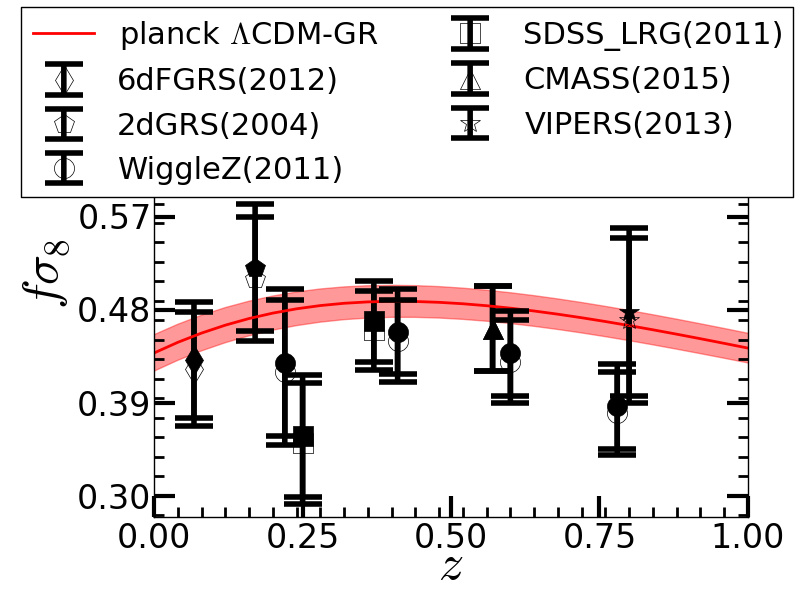
\includegraphics[width=0.5\textwidth]{plots/fs8z_data_bestfit.png}
\caption{The measured $f\sigma_8$ from different survey covering redshift range $0.06<z<0.8$. The empty markers represents the reported measurement of $f\sigma_8$ and the filled marker are for the corrected values for Planck Comsology. The red band shows the Planck $1\sigma$ prediction. }
\label{fig:fs8z}
\end{figure}

\begin{figure}
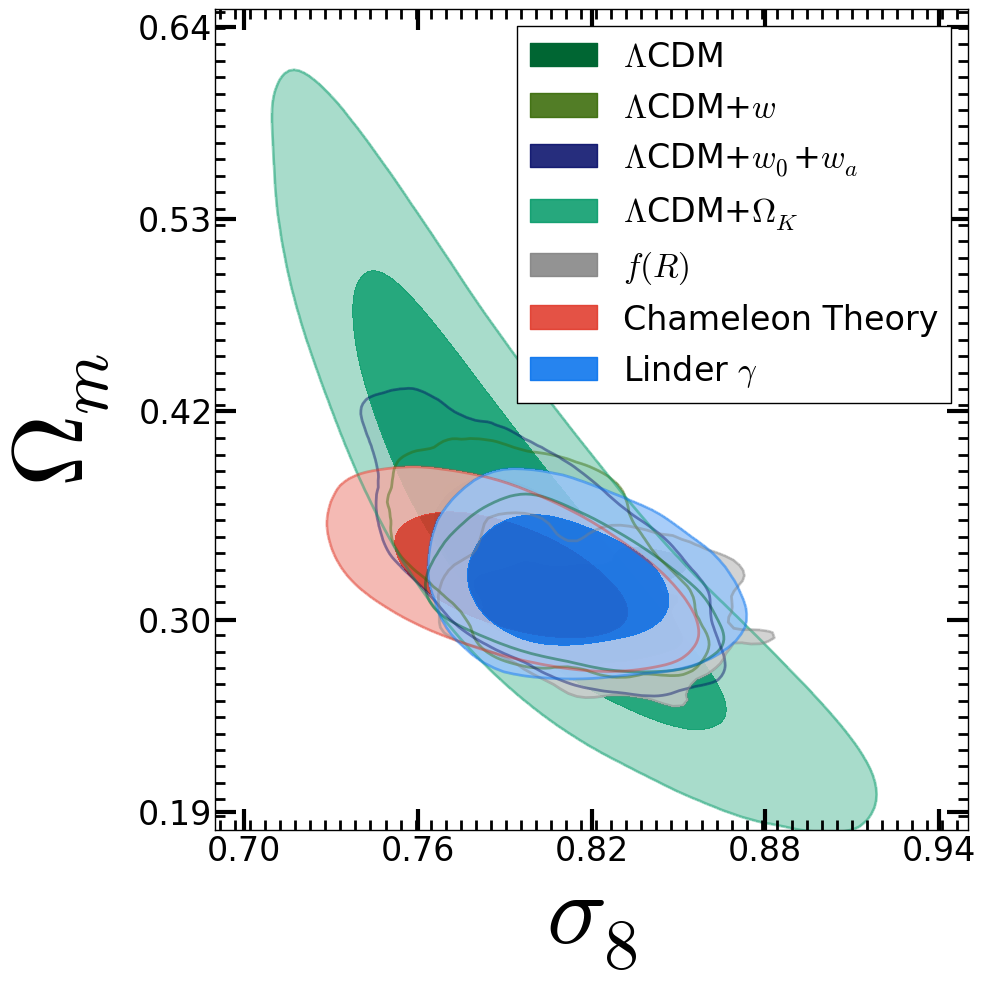
\includegraphics[width=0.5\textwidth]{plots/Like-2D/All-sigma8-omegam_2D.png}
\caption{The figure shows the $1\sigma$ and $2\sigma$ region for each of the model consider in this paper in $\Omega_m$-$\sigma_8$ plane. It shows that the posterior likelihood is consistent for each of the model in this parameter space. All the model have similar constraint in this space except kCDM.}
\label{fig:Ms8}
\end{figure}


We have combine CMB data set and measurement of growth from various redshift survey in order to constrain the parameters of standard cosmology ($\Lambda$CDM), extended cosmology models  and modified gravity. For all the models considered in this paper our analysis gives consistent constraint for the standard $\Lambda$CDM parameters (\{$\Omega_b h^2, \Omega_c h^2, 100\Theta_{MC} ,\tau, n_s, log(10^{10} A_s) $\}).  The Figure \ref{fig:Ms8} shows the constraint on $\Omega_m$- $\sigma_8$ plane for $\Lambda$CDM, wCDM, kCDM, $f(R)$ ,Chameleon gravity and Linder $\gamma$ parametrization.  All the model gives similar precision for this parameter space except the kCDM model. The possibility of having non-zero spatial curvature expand the feasible region in $\Omega_m$-$\sigma_8$.  

\subsection{$\Lambda$CDM-GR}
The Figure \ref{fig:LCDM} shows the one dimensional marginalized likelihood for standard $\Lambda$CDM-GR cosmology. Our parameter contraints are completely consistent with the planck 2013 results. Adding measurement of growth rate with planck contraint doesn't improve the precision of cosmology because the precision of planck prediction (pink band in Figure \ref{fig:fs8z})  is much smaller than the precision of the measurement of growth factor (black points in Figure \ref{fig:fs8z}). 

%We see \textcolor{red}{x} $\sigma$ deviation in $\sigma_8$ which points toward slight tension in the measurement of $\sigma_8$ between various measurement (add reference).

\begin{figure*} 
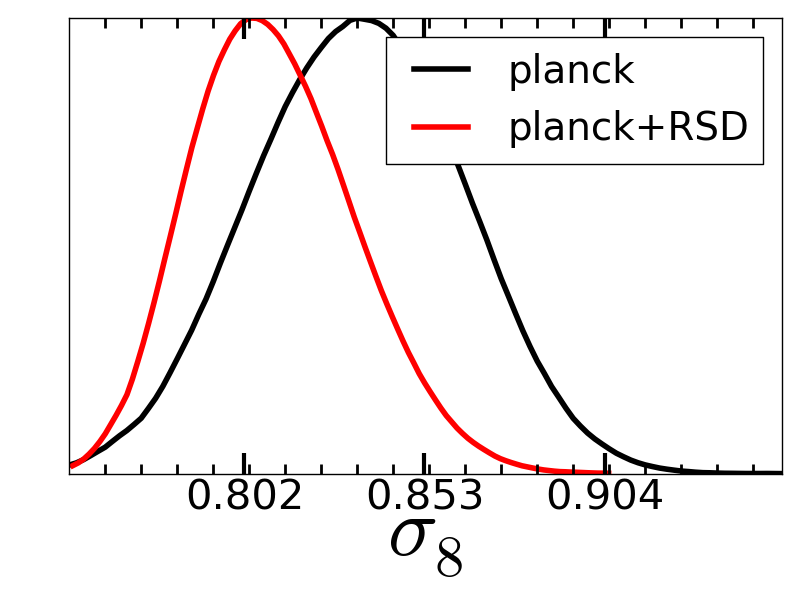
\includegraphics[width=0.3\textwidth]{plots/planck-RSD-GR-sigma8.png}
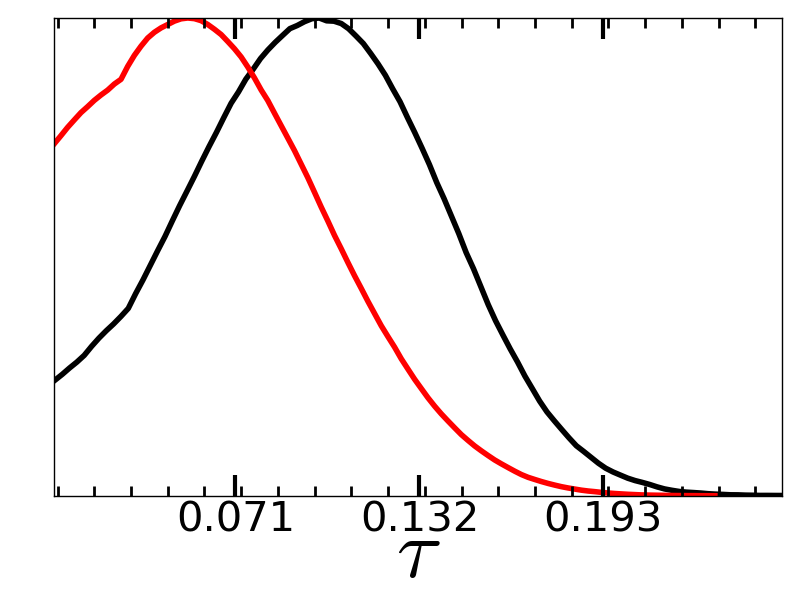
\includegraphics[width=0.3\textwidth]{plots/planck-RSD-GR-tau.png}
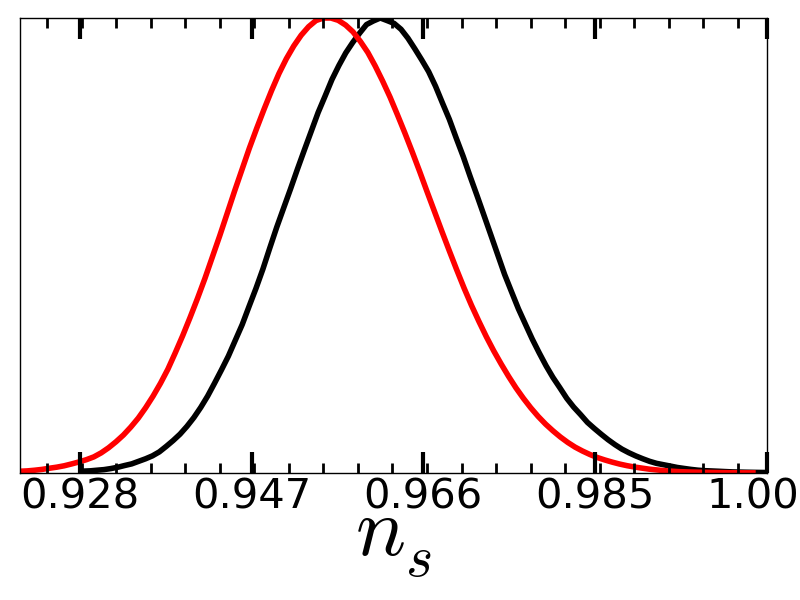
\includegraphics[width=0.3\textwidth]{plots/planck-RSD-GR-ns.png}
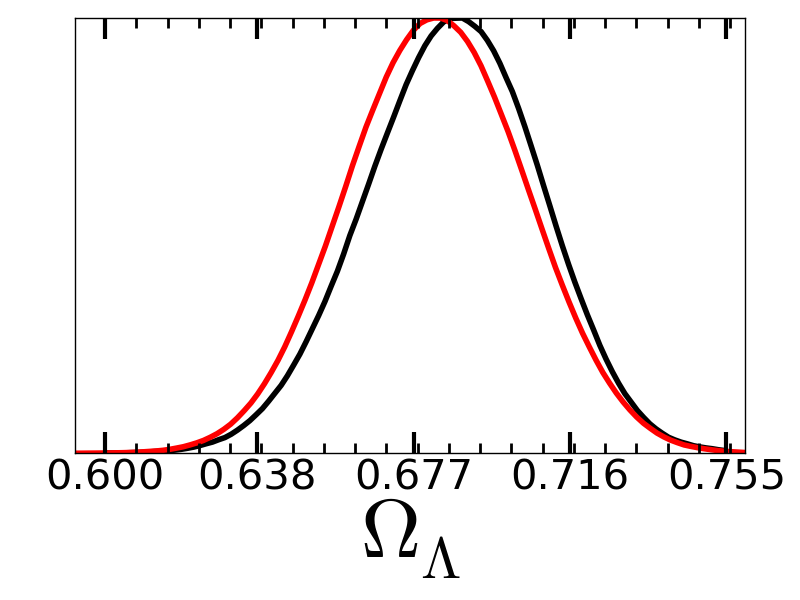
\includegraphics[width=0.3\textwidth]{plots/planck-RSD-GR-omegal.png}
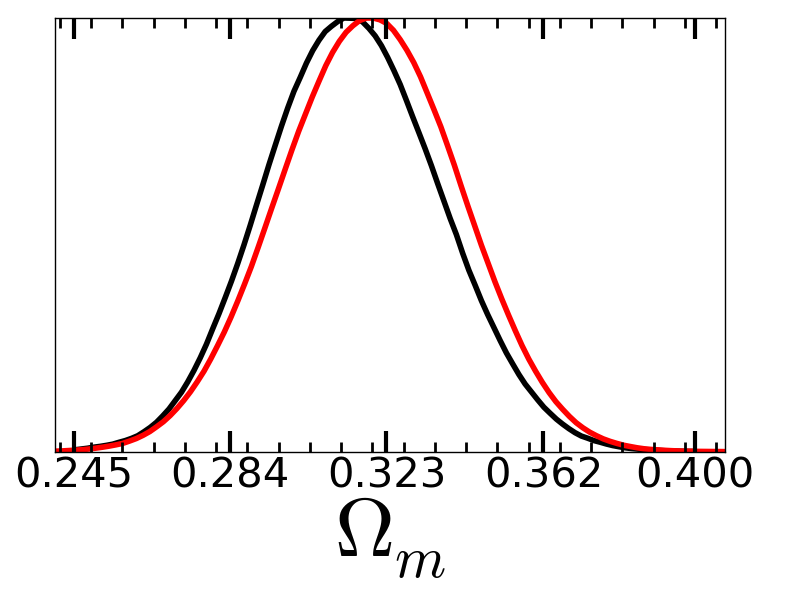
\includegraphics[width=0.3\textwidth]{plots/planck-RSD-GR-omegam.png}
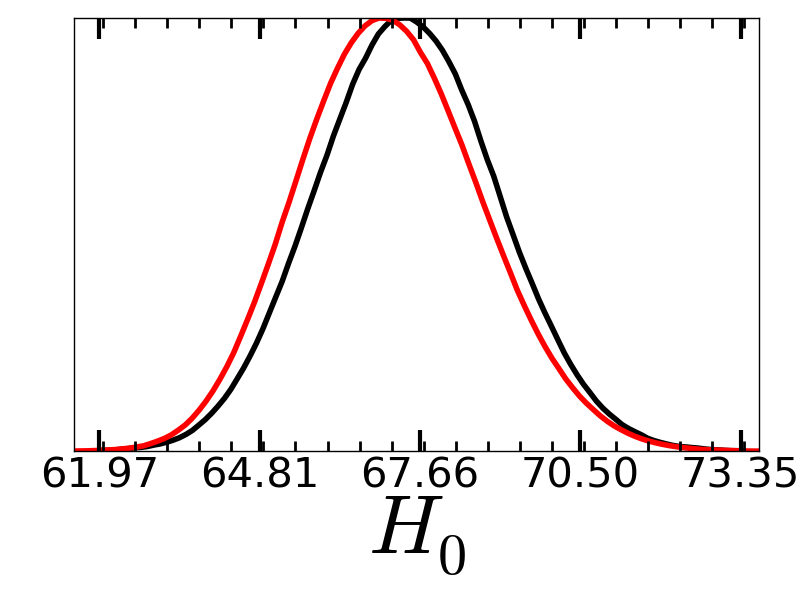
\includegraphics[width=0.3\textwidth]{plots/planck-RSD-GR-H0.png}
\caption{ $\Lambda$CDM-GR: We use GR as the model for gravity to determine the growth factor and fit for $f\sigma_8$ measurement with planck likelihood. The two most prominent effect are in optical depth $\tau$ and scalar amplitude of primordial power spectrum $A_s$. Which is also reflected in the derived parameter $\sigma_8$ and mid redshift of re-ionization $z_{re}$.}
\label{fig:LCDM}
\end{figure*}

\subsection{Dark Energy Equation of state ($w$CDM)}
\begin{figure}
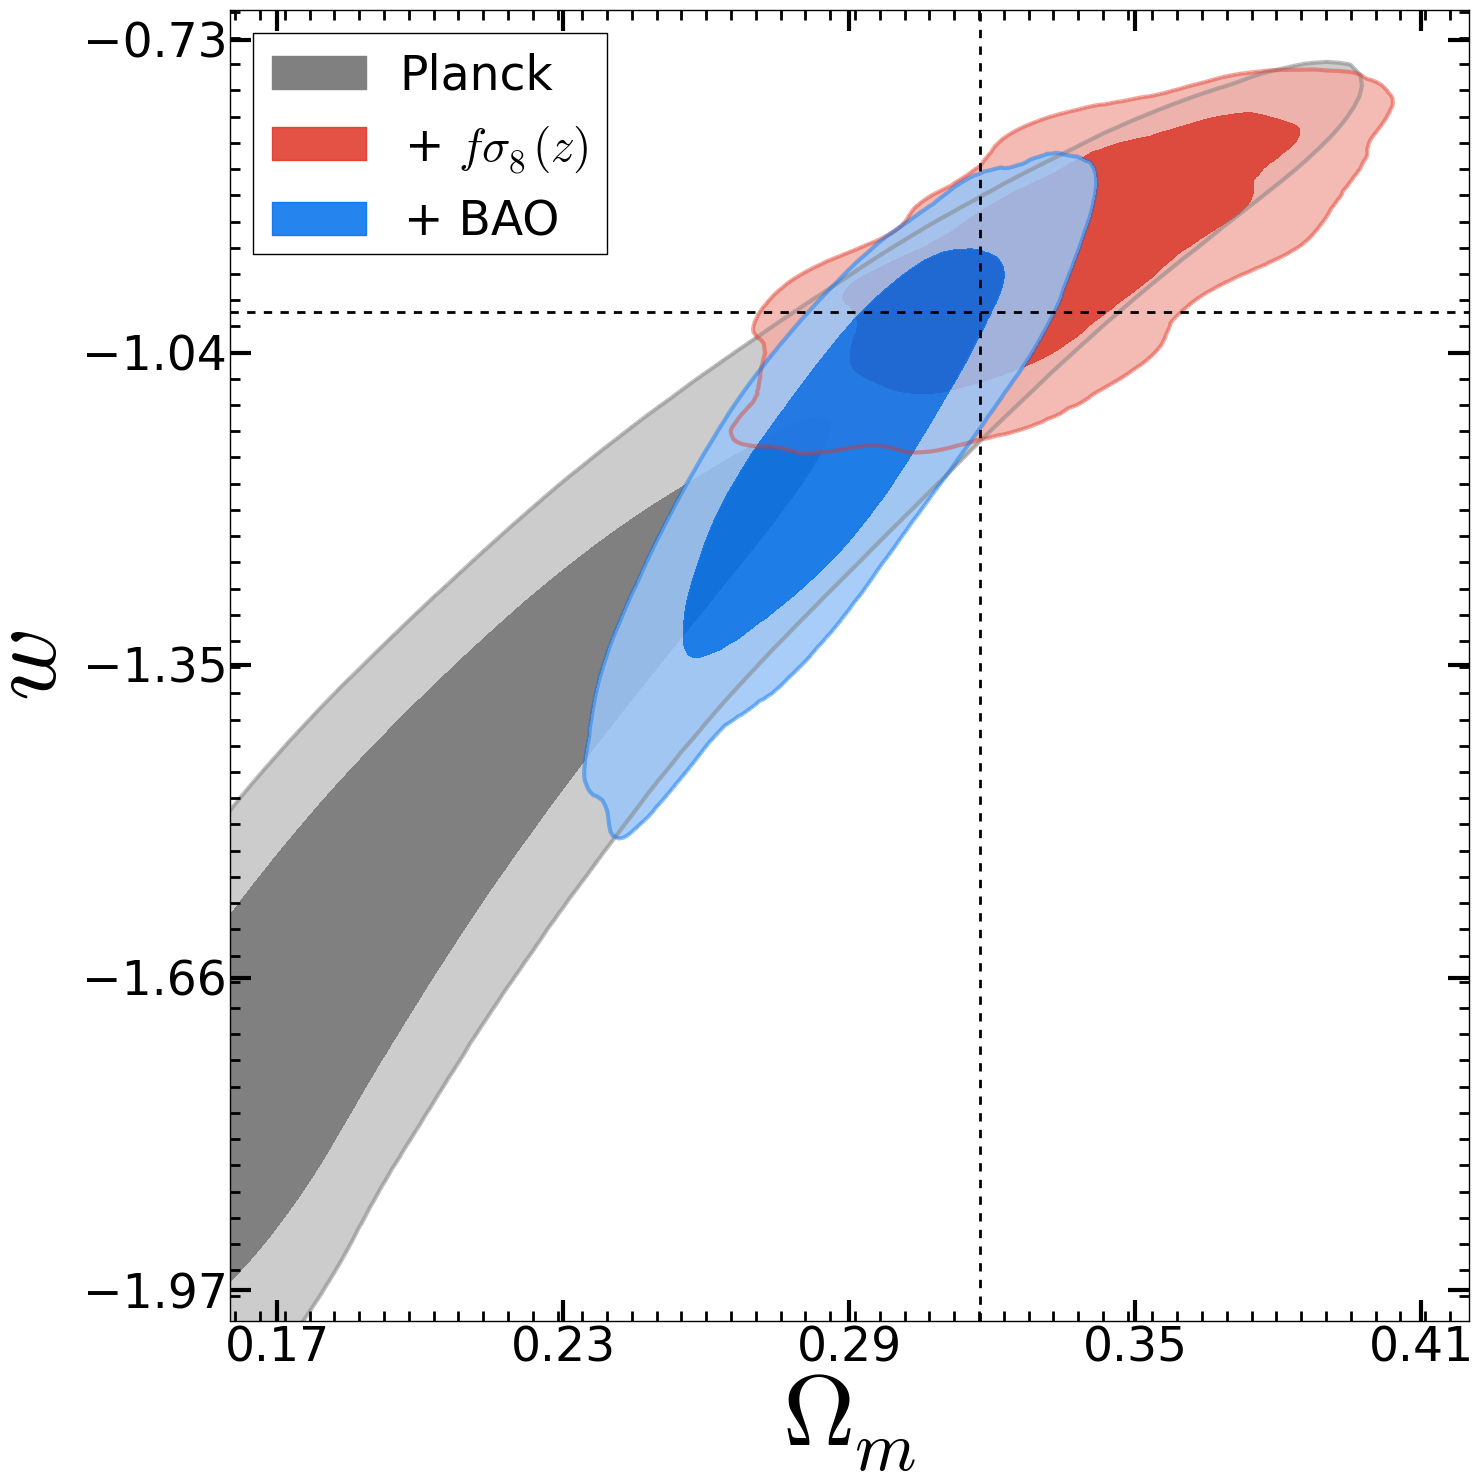
\includegraphics[width=0.5\textwidth]{plots/Like-2D/wCDM-omegam-w_2D.png}
\caption{The two dimensional posterior likelihood $w$ and $\Omega_m$  for $w$CDM. The grey contour is for Planck, blue contour is combined constraint from Planck and BAO. The red contour represents  our results while combining Planck with $f\sigma_8$.}
\label{fig:wCDM}
\end{figure}

We have looked at the $w$CDM (one parameter extension of $\Lambda$CDM) , where w is the dark energy equation of state.
The Figure \ref{fig:wCDM} shows the two dimensional likelihood of of $w$ and $\Omega_m$. The grey contour are planck only contraint, blue contour shows planck combined with the BAO (Baryon Acoustic Oscillation cite paper) measurement  and red contours are our result planck combined with growth factor ($f\sigma_8$) measurement. We obtain $w=x \pm y$ (z\% measurement) which is consistent fiducial value of $w=-1$ for $\Lambda$CDM. The constraint we obtained is similar in precision as compared to BAO but has different degeneracy. Therefore combining planck with BAO and RSD together might give a much stronger constraint on dark energy equation of state w.  But, That will require taking care of covariances between the BAO and RSD and they come from exactly same galaxy sample.

\subsection{Time-dependent Dark Energy ($w_0 w_a$CDM)}
\begin{figure}
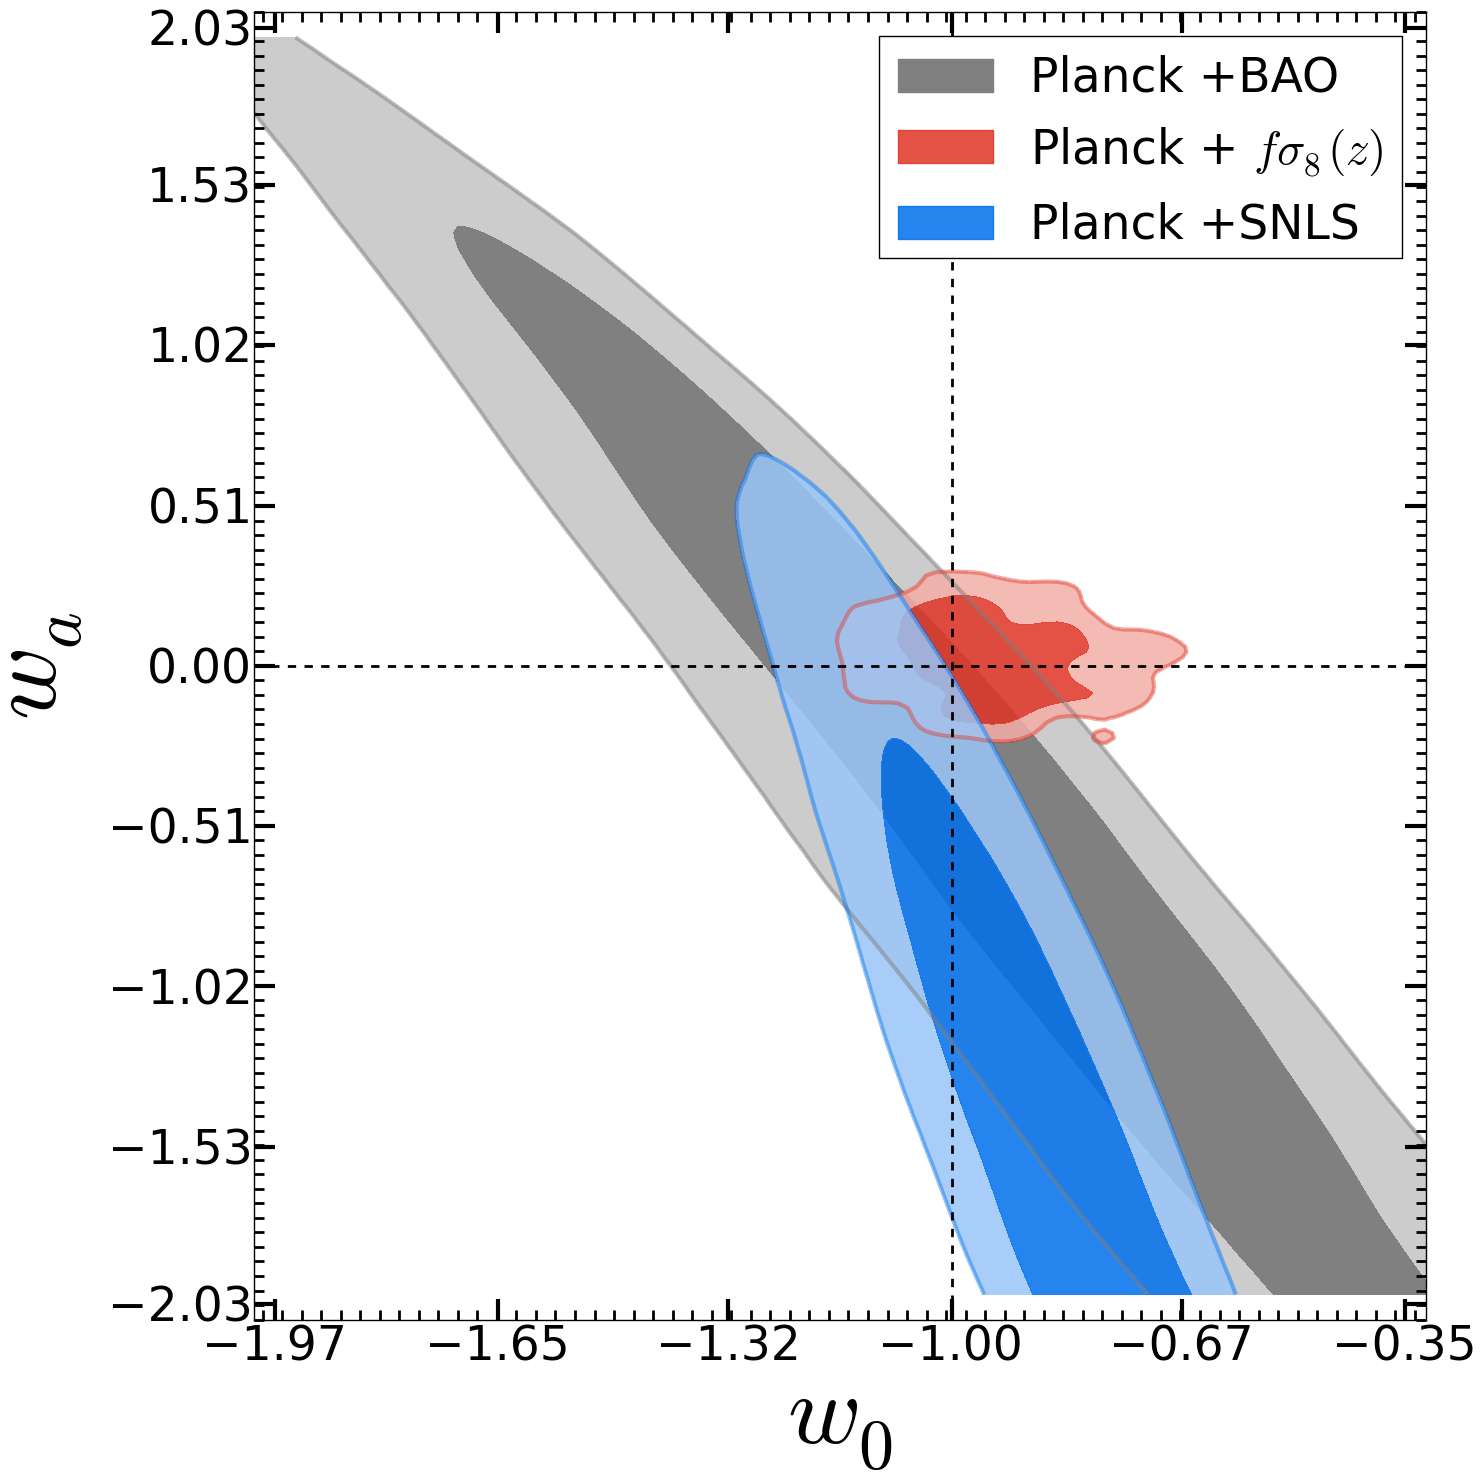
\includegraphics[width=0.5\textwidth]{plots/Like-2D/w0wa-w-wa_2D.png}
\caption{The two dimensional posterior likelihood of $w_0$ and $w_a$  for time-dependent extension. The grey contour is for Planck, blue contour is combined constraint from Planck and BAO. The red contour represents  our results while combining Planck with $f\sigma_8$.}
\label{fig:w0waCDM}
\end{figure}

The $w$CDM model which propose a constant dark energy is limited in its physical characteristic. Many model propose time-dependent which is popularly tested using linear relation $w(z)=w_0 +w_a \frac{z}{1+z}$ with $w_0$ and $w_a$ as free parameter. This captures the slowly rolling minimally-coupled scalar field, low-redshift behavior of light. The dynamical evolution of $w(z)$ can change the growth factor significantly and leave a imprint on the CMB. The combination of CMB and collection of growth factor at different redshift is a unique way to test the time-dependent dark energy model.

Figure \ref{fig:w0waCDM} shows the $1\sigma$ and $2\sigma$ region for ($w_0,w_a$). The grey contour is from the combination of Planck and BAO. The blue contours is from Planck and SNLS. The red contour is our measurement by combining the growth rate measurements with Planck. The $\Lambda$CDM-GR prediction $(w_0,w_a)=(-1,0)$ is completely consistent with our posterior. We have obtained constraint on $w_0=x \pm y$ (z\% measurement) and $w_a=x \pm y$ (z\% measurement) which is much stronger constraint than the existing measurements.


\subsection{Spatial Curvature (kCDM)}
\begin{figure}
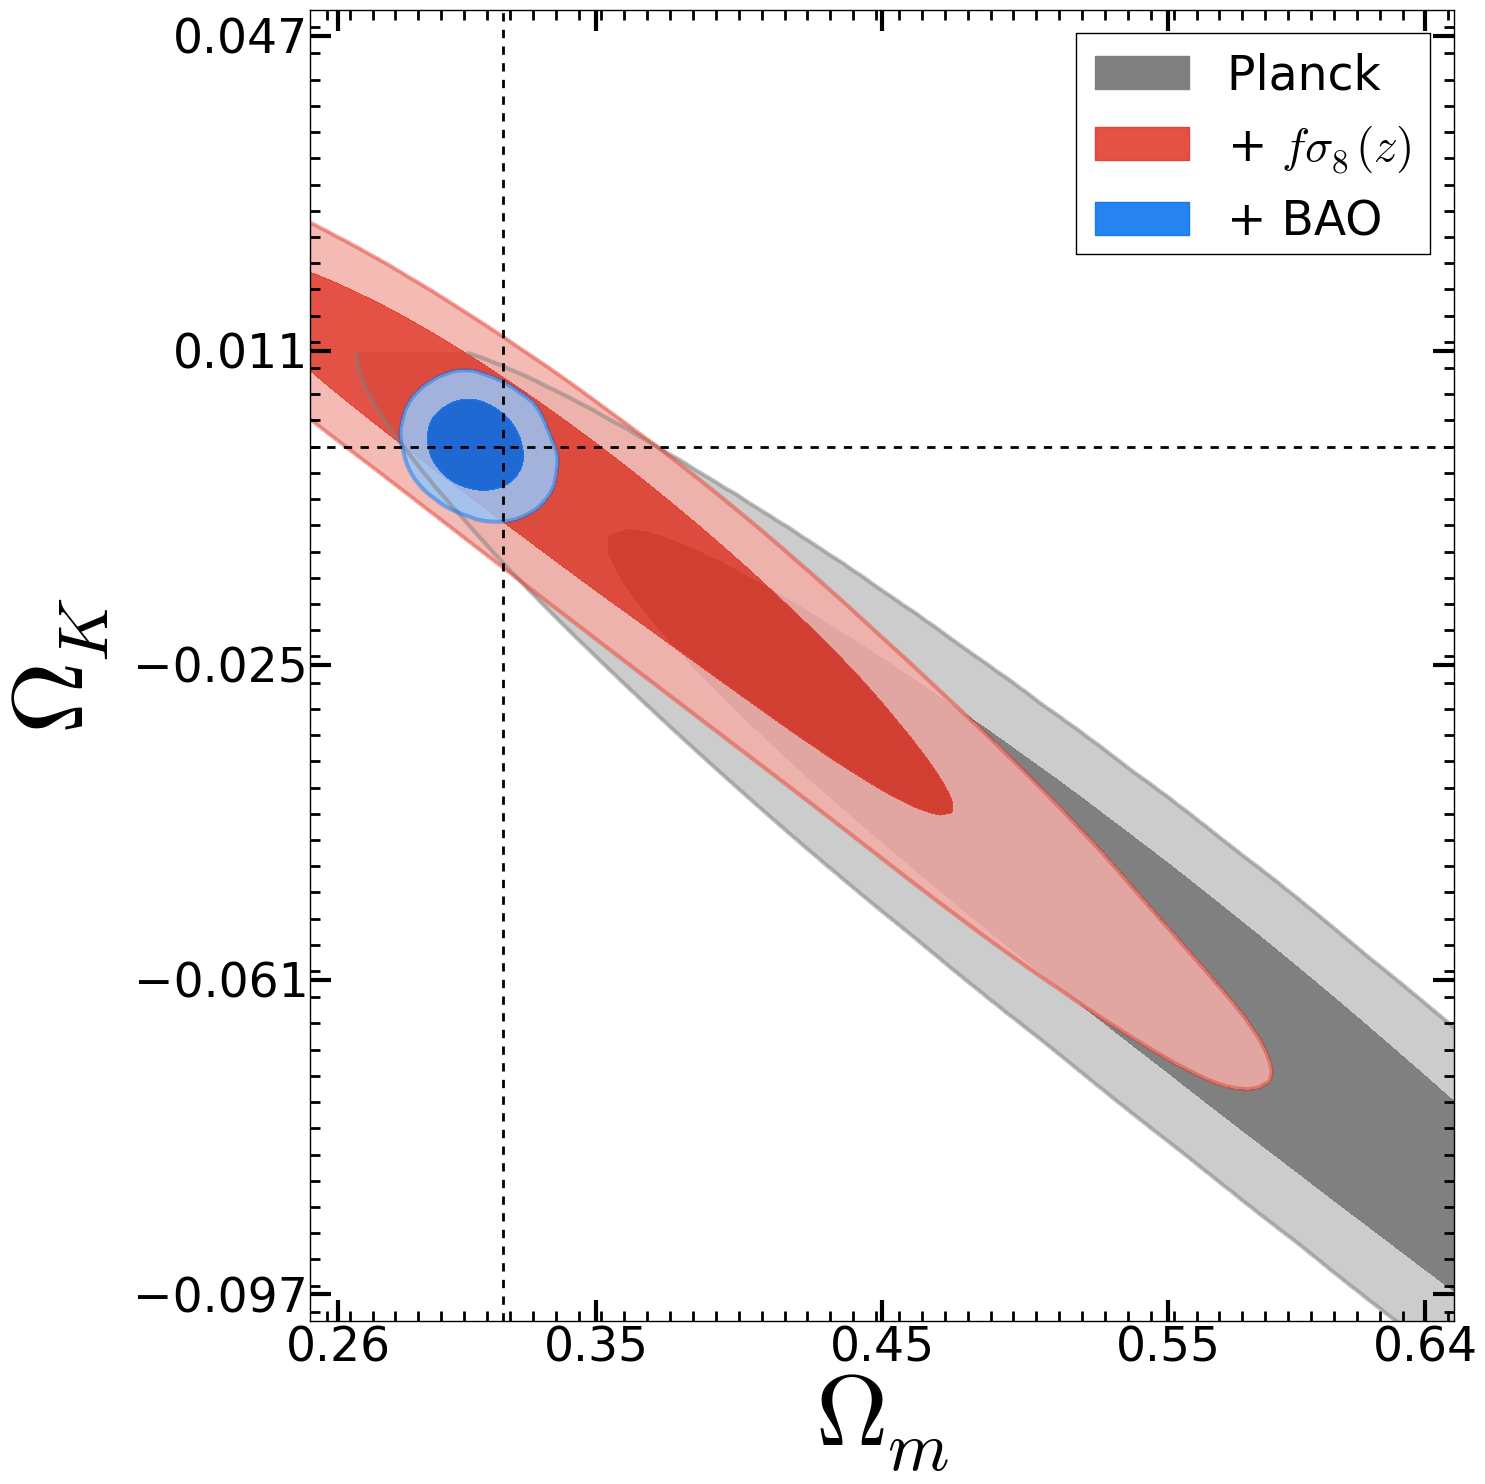
\includegraphics[width=0.5\textwidth]{plots/Like-2D/kCDM-omegam-omegak_2D.png}
\caption{The two dimensional posterior likelihood of $\Omega_k$ and $\Omega_m$  for kCDM. The grey contour is for Planck, blue contour is combined constraint from Planck and BAO. The red contour represents  our results while combining Planck with $f\sigma_8$}
\label{fig:kCDM}
\end{figure}

We consider a model with spatial curvature parametrized with $\Omega_K$ as free parameter called kCDM along with $\Lambda$CDM parameters. The Figure \ref{fig:kCDM} shows the posterior for the $\Omega_K$ and $\Omega_m$ plane. We measure $\Omega_K= x \pm y$ (z \% measurement) shown by red shaded region by combining planck and $f\sigma_8(z)$ measurement.The grey region is using planck only measurement which gives $\Omega_K= x \pm y$ (z \% measurement). The blue shaded region represents the constraint from planck and BAO combined. The BAO is much superior probe to constrain the spatial curvature of the universe compared to RSD. It will be interesting to see if RSD and BAO combined will give any different result.


\subsection{Chameleon Gravity}
\begin{figure}
    \begin{center}        
        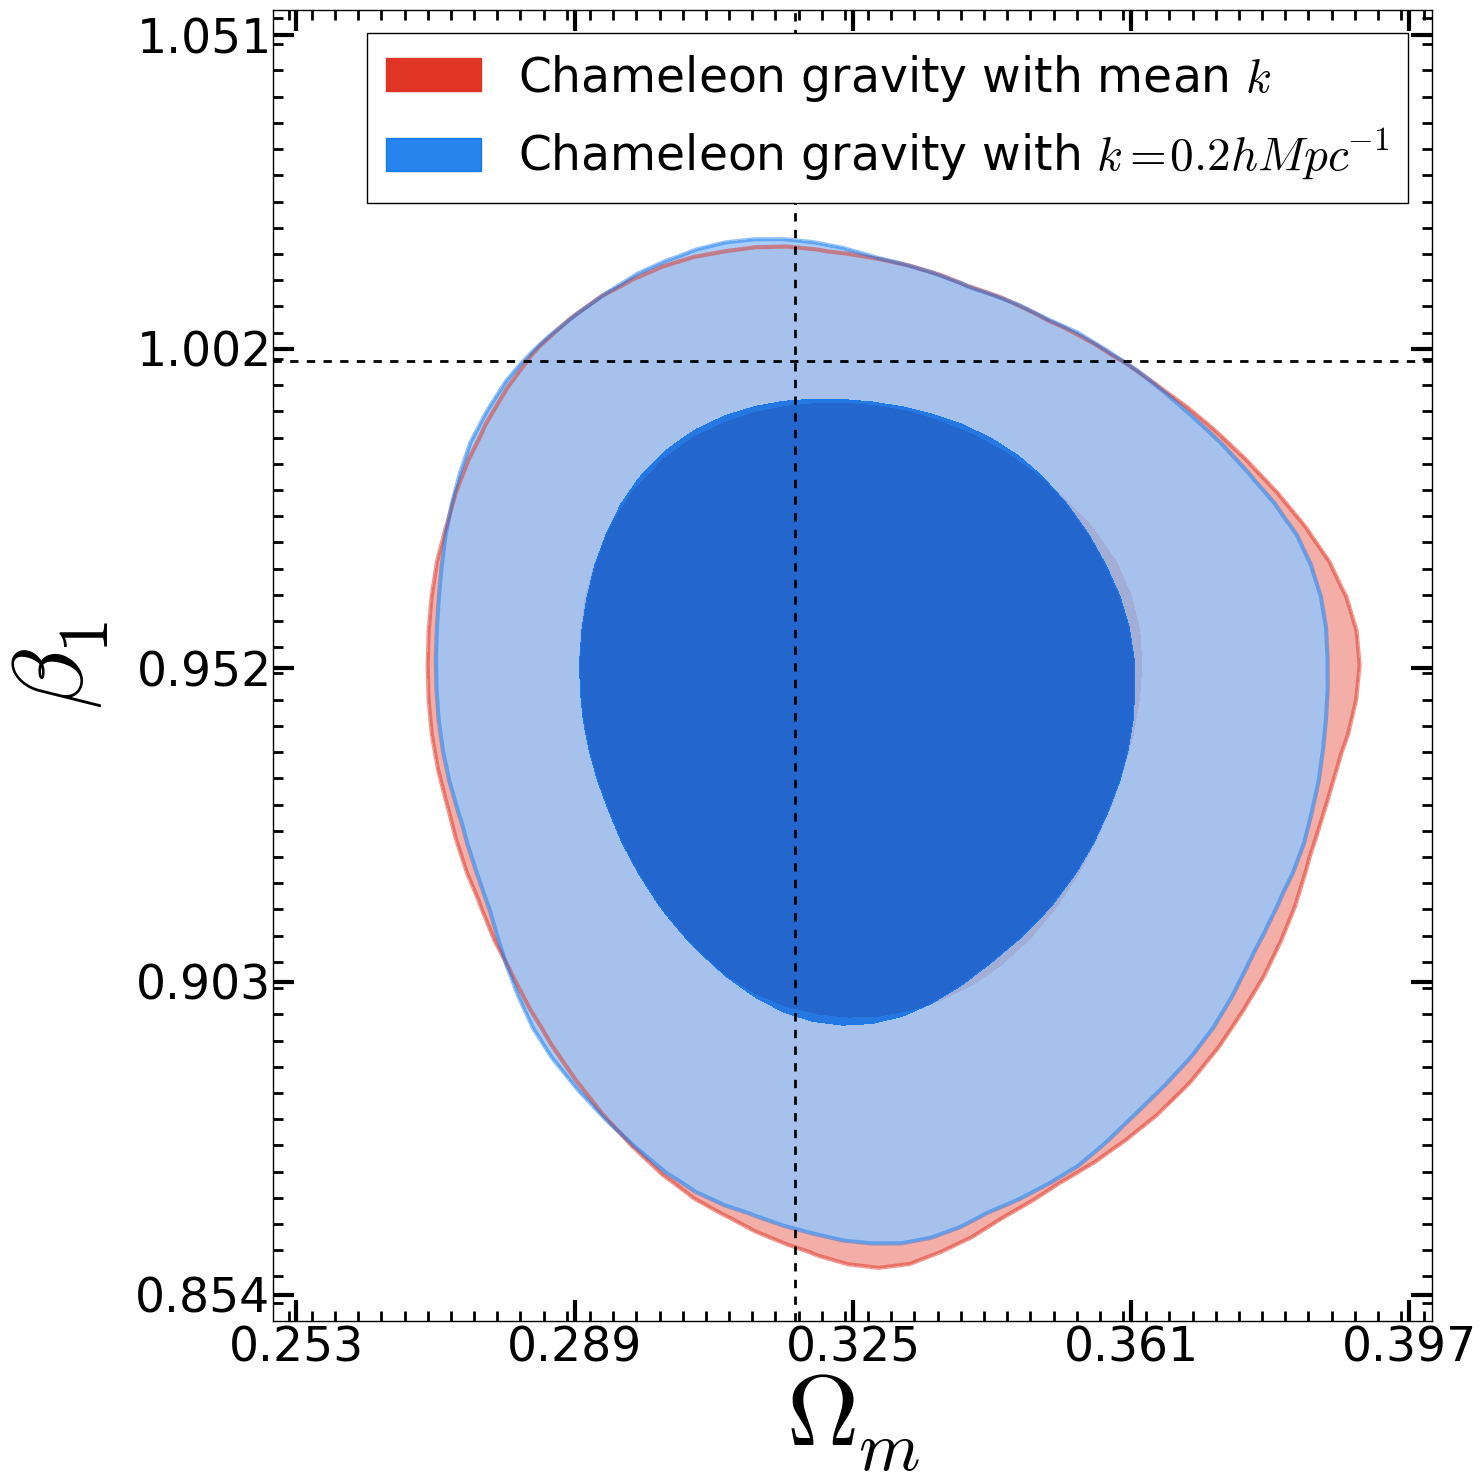
\includegraphics[width=0.5\textwidth]{plots/Like-2D/ChamB1-omegam-B1_2D.png}
     \end{center}
     \caption{Chameleon}
     \label{fig:Chambeta}
\end{figure}

The three parameters of Chameleon gravity ($\beta_1, B_0, s$) is constrained with the standard $\Lambda$CDM parameters using planck and $f\sigma_8(z)$ measurement. The Chameleon theory predicts a scale dependent growth rate ($f\sigma_8(k,z)$) where as the measurement are at some effective $k$. We have used two different approach to incorporate the k-dependence in our analysis. The Figure \ref{fig:Chambeta} shows the two dimensional posterior in $\beta_1$ and $\Omega_m$ plane. The blue contours are likelihood while evaluating the growth rate at an effective $k$ where red contour is for the case when we use effective growth rate which is averaged over scales used in the actual $f\sigma_8$ measurement. We obtained $\beta_1= x \pm y$ (z \% measurement), which is an improvement by a factor of X on the previous constraint $\beta_1= x \pm y$ (z \% measurement) using power spectrum (cite the Alireza paper). The growth rate constrain the other two parameter $B_0$ and $s$ of the model very weakly. You can see some of the contours in Appendix (add an appendix for this part).

%\begin{figure*} 
%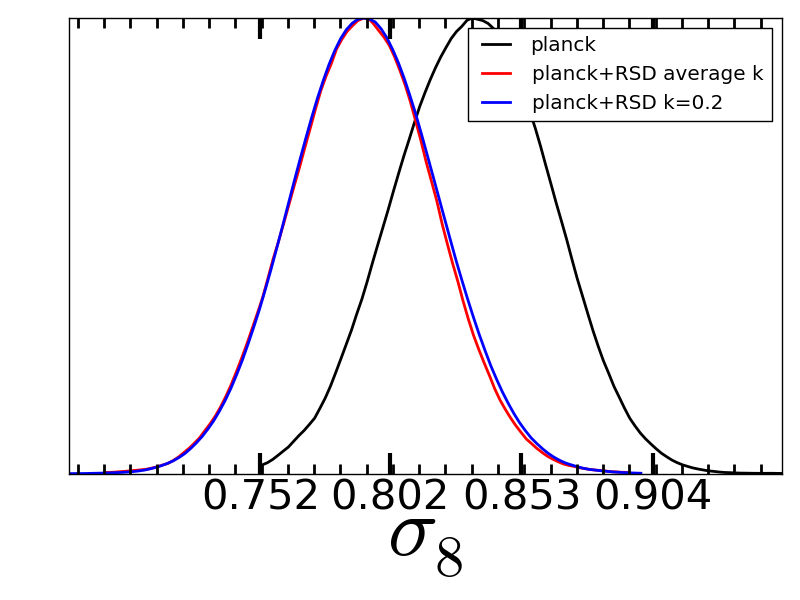
\includegraphics[width=0.3\textwidth]{plots/planck-RSD-Cham-sigma8.png}
%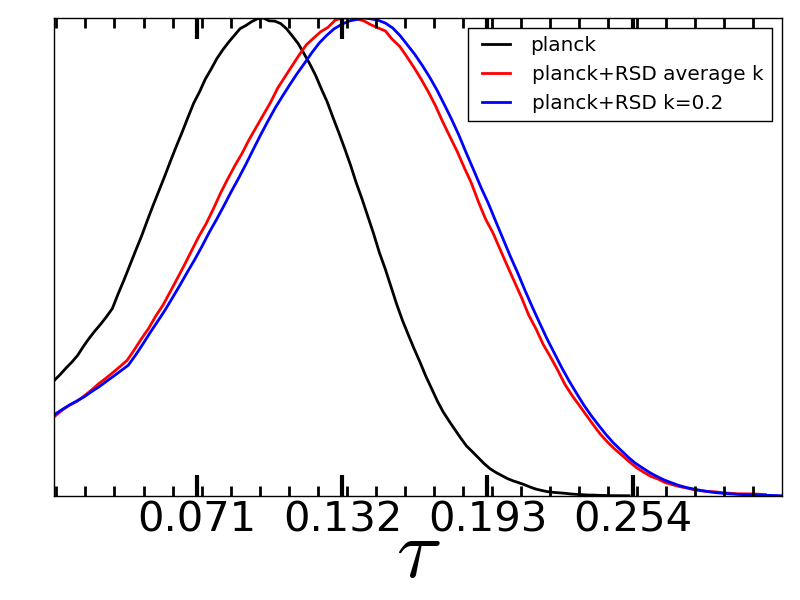
\includegraphics[width=0.3\textwidth]{plots/planck-RSD-Cham-tau.png}
%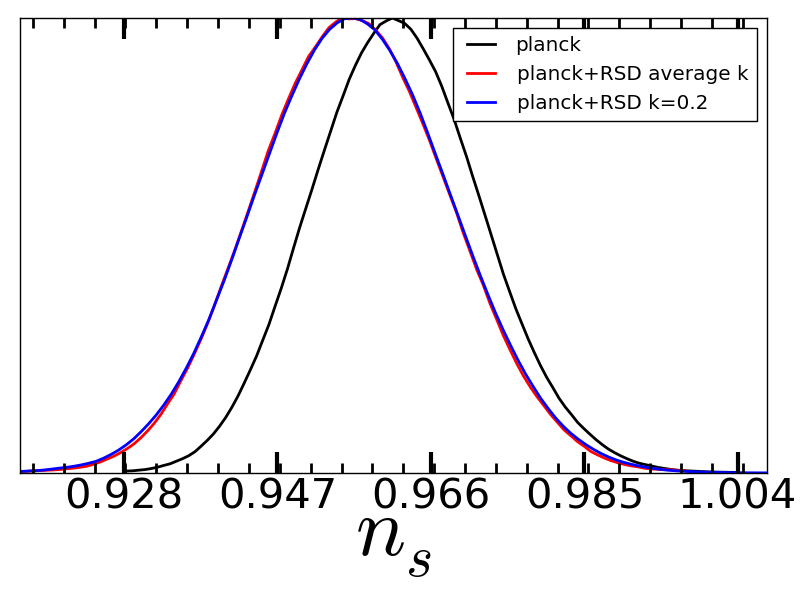
\includegraphics[width=0.3\textwidth]{plots/planck-RSD-Cham-ns.png}
%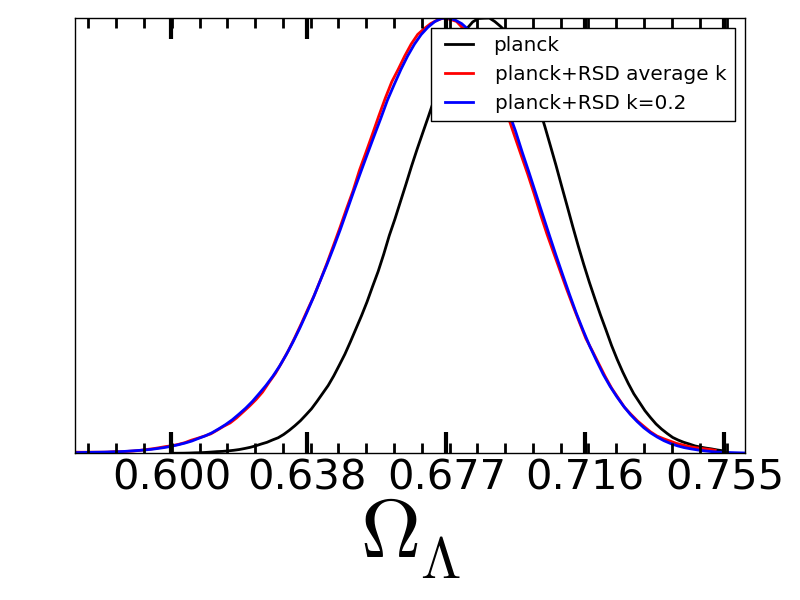
\includegraphics[width=0.3\textwidth]{plots/planck-RSD-Cham-omegal.png}
%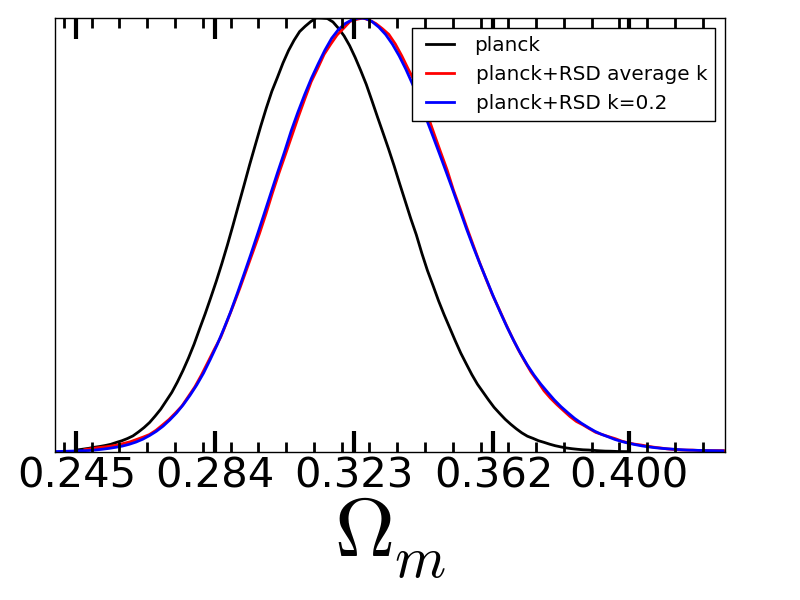
\includegraphics[width=0.3\textwidth]{plots/planck-RSD-Cham-omegam.png}
%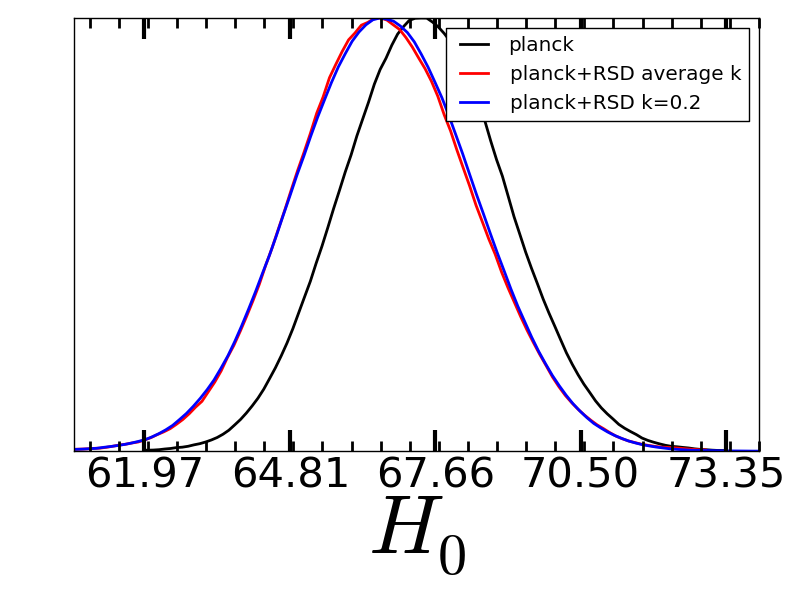
\includegraphics[width=0.3\textwidth]{plots/planck-RSD-Cham-H0.png}
%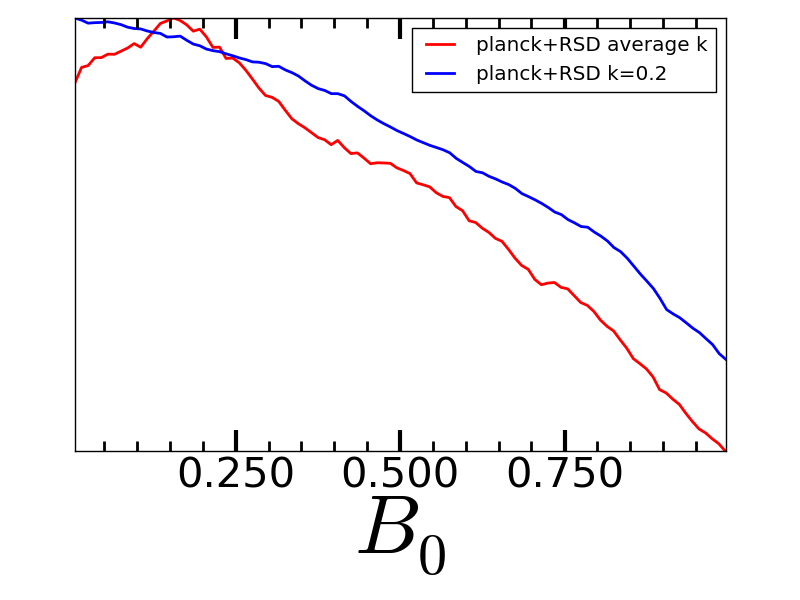
\includegraphics[width=0.3\textwidth]{plots/planck-RSD-Cham-lambda1_2.png}
%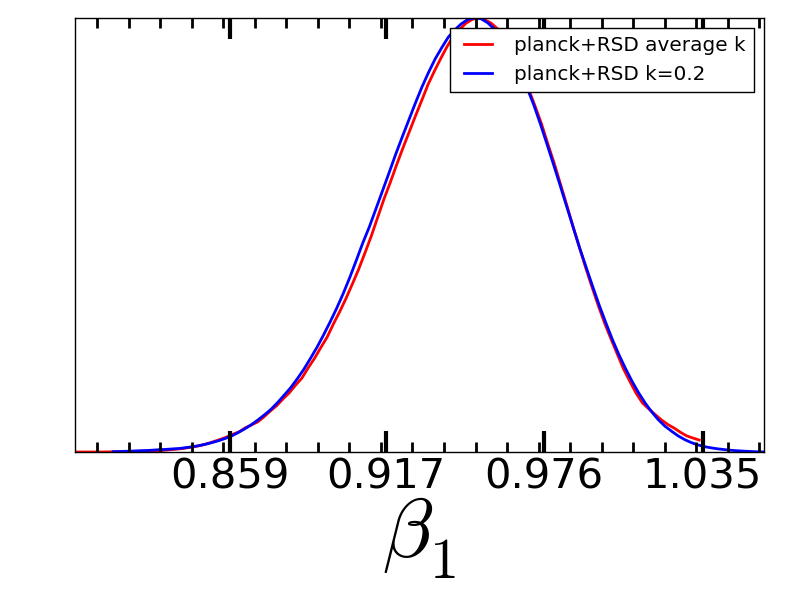
\includegraphics[width=0.3\textwidth]{plots/planck-RSD-Cham-B1.png}
%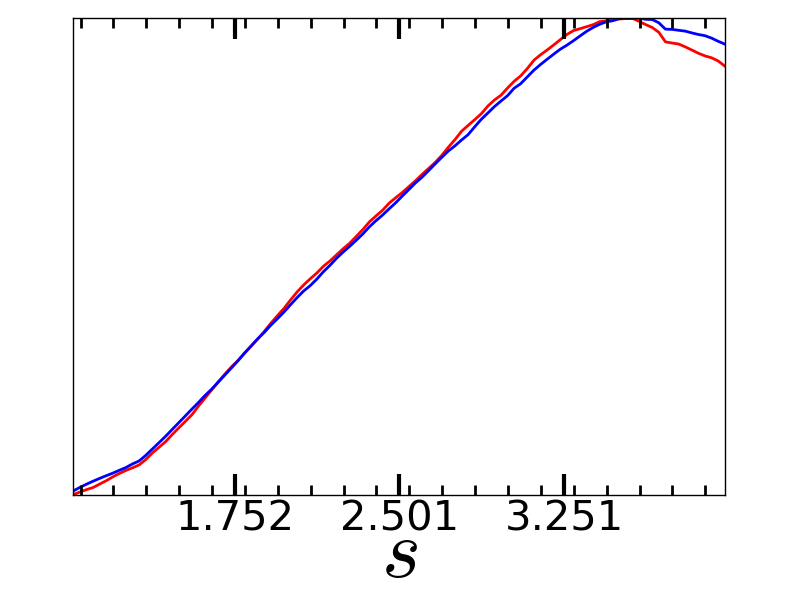
\includegraphics[width=0.3\textwidth]{plots/planck-RSD-Cham-ss.png}
%\caption{Chameleon type theory(Yukawa model): This is the three parameter model \{$\beta_1, B_o, s$\}, The growth factor seems to be constraining mostly $\beta_1=0.945 \pm 0.031$ and have very weak constraint on other two parameters $B_o=0.45 \pm 0.30 , s=2.94 \pm 0.75$}
%\end{figure*}

\subsection{Linder's $\gamma_L$ parametrization}
\begin{figure}
    \begin{center}        
        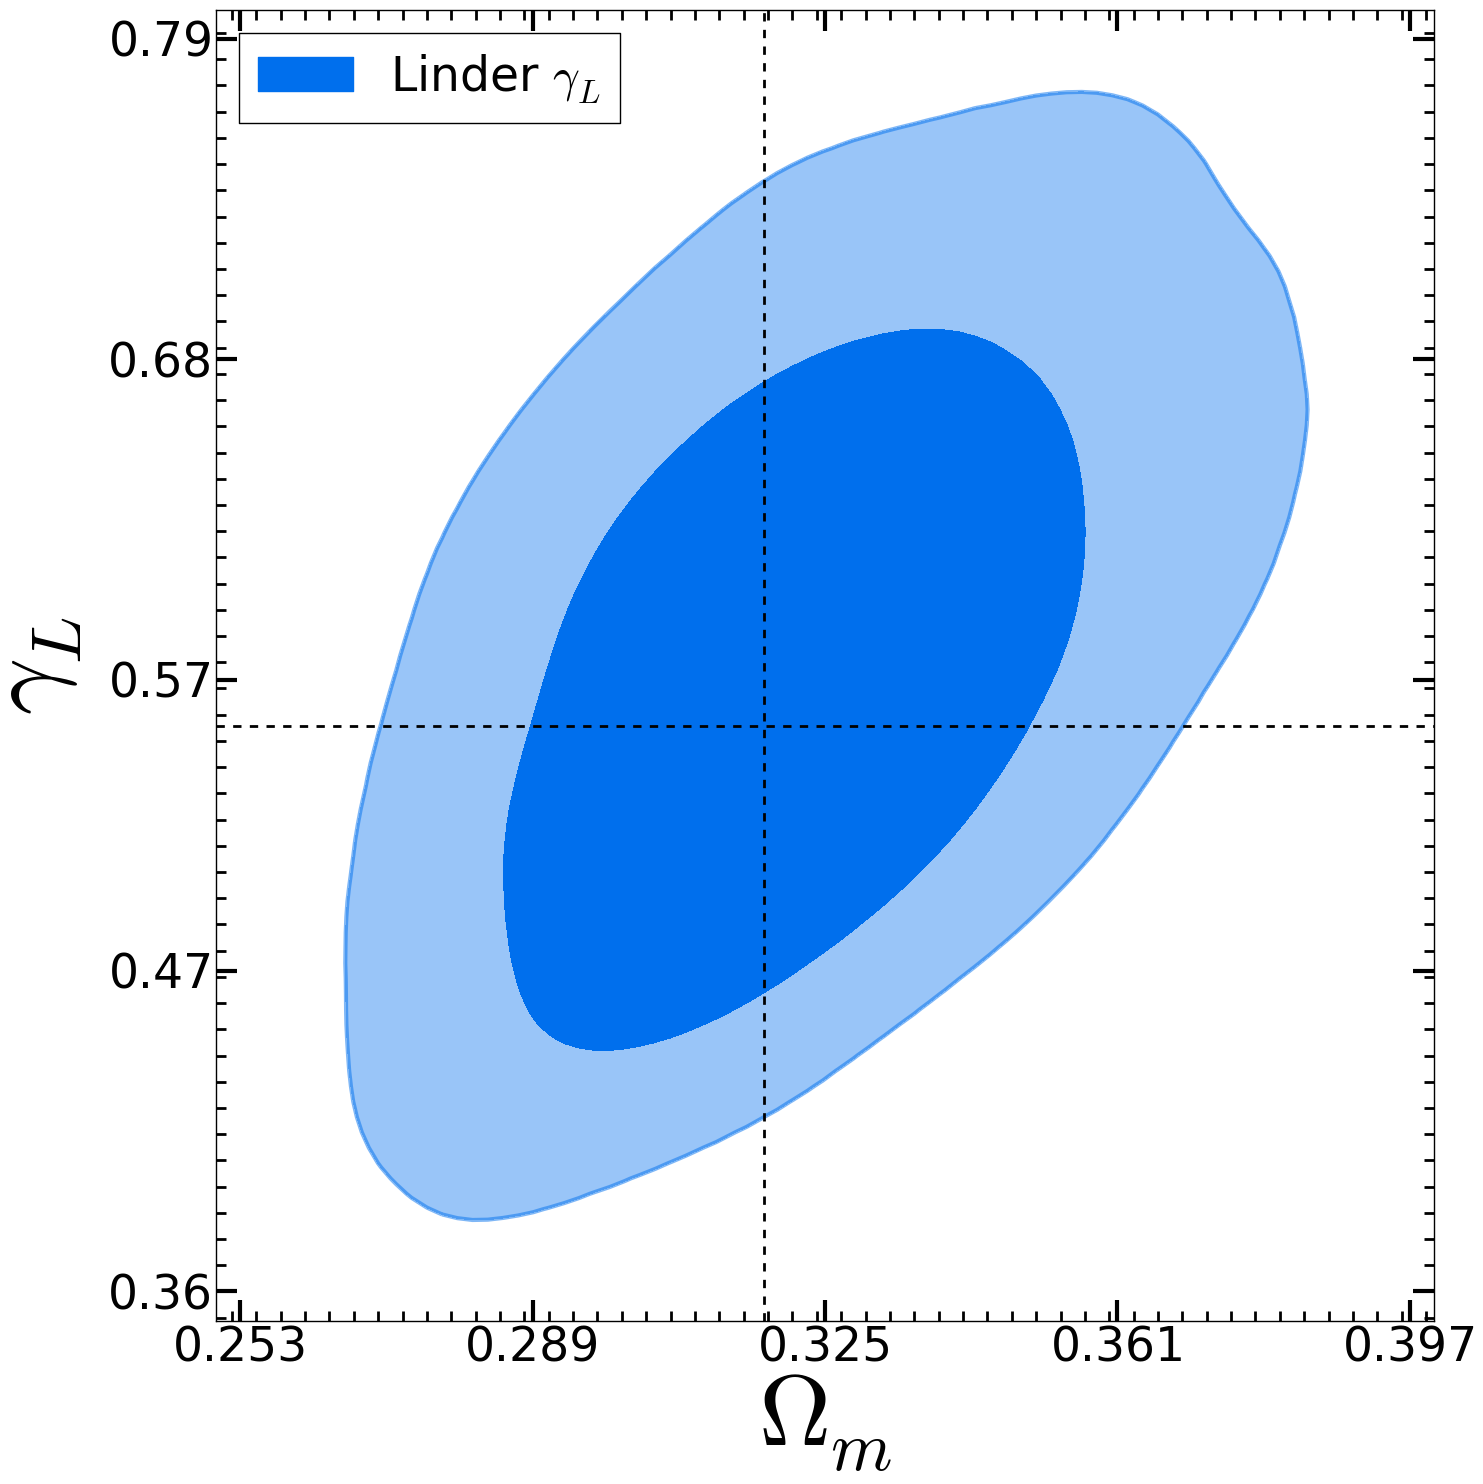
\includegraphics[width=0.5\textwidth]{plots/Like-2D/Lind-omegam-Linder_gamma_2D.png}
     \end{center}
     \caption{Linder}
     \label{fig:Linder}
\end{figure}

The general theory of relativity predicts the precise value of growth factor in the linear regime to be $f=\Omega_m^{0.545}$.  In order to test the deviations from GR we have parameterized the growth factor using Linder $\gamma_L$ ( cite Linder \& Cahn 2008) as $f=\Omega_m^{\gamma_L}$. The marginalized two dimensional likelihood for $\Omega_m$ and $\gamma_L$ is shown in Figure \ref{fig:Linder}. We have obtained $\gamma_L = x \pm y$ (z\% measurement) completely consistent with the general relativity prediction.

%\begin{figure*} 
%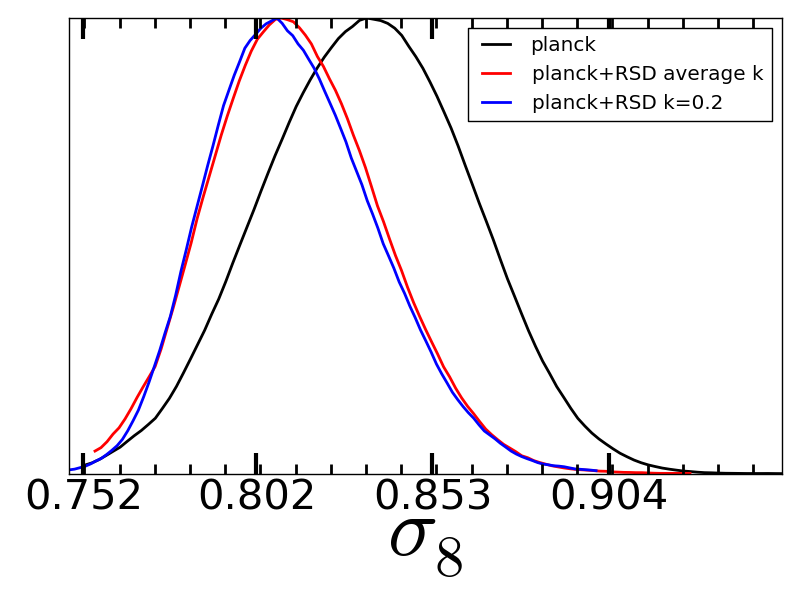
\includegraphics[width=0.3\textwidth]{plots/planck-RSD-Lind-sigma8.png}
%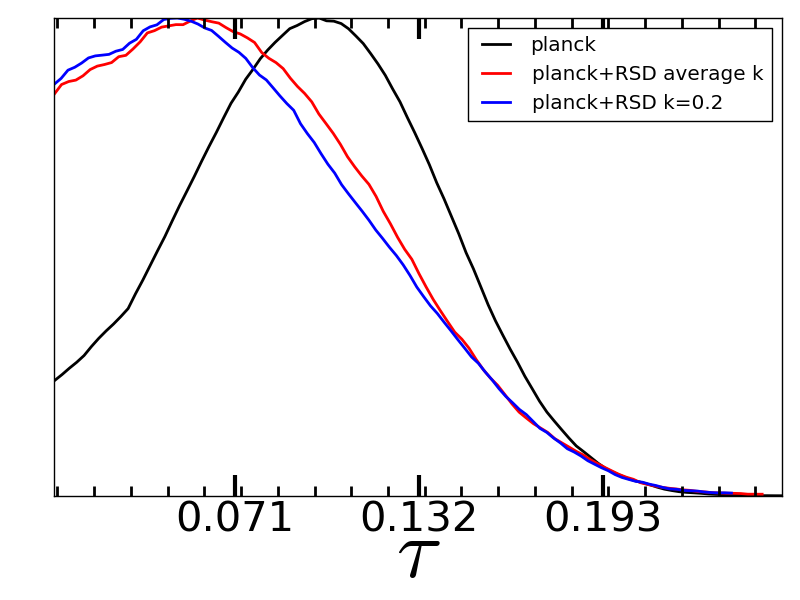
\includegraphics[width=0.3\textwidth]{plots/planck-RSD-Lind-tau.png}
%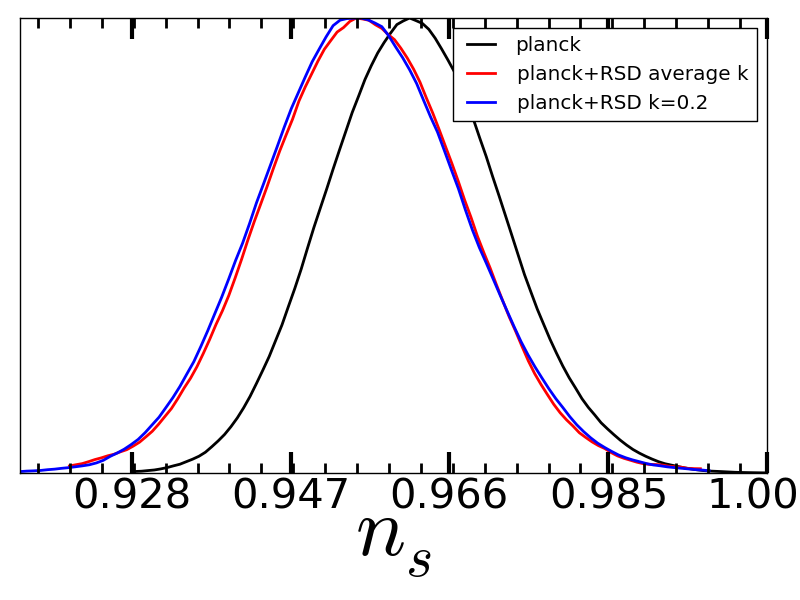
\includegraphics[width=0.3\textwidth]{plots/planck-RSD-Lind-ns.png}
%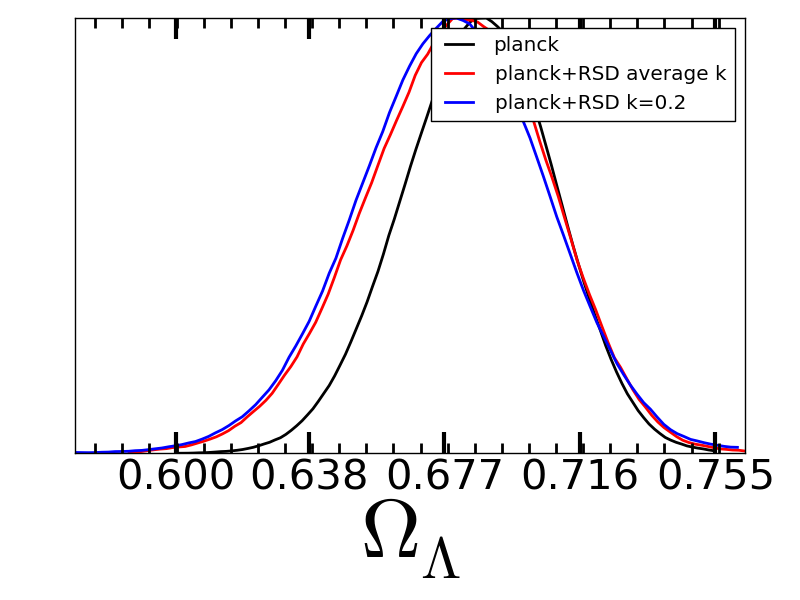
\includegraphics[width=0.3\textwidth]{plots/planck-RSD-Lind-omegal.png}
%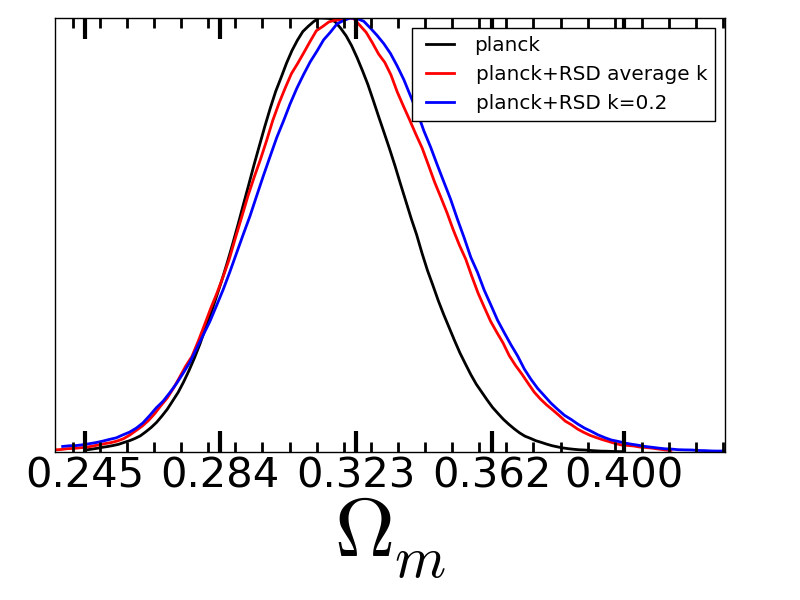
\includegraphics[width=0.3\textwidth]{plots/planck-RSD-Lind-omegam.png}
%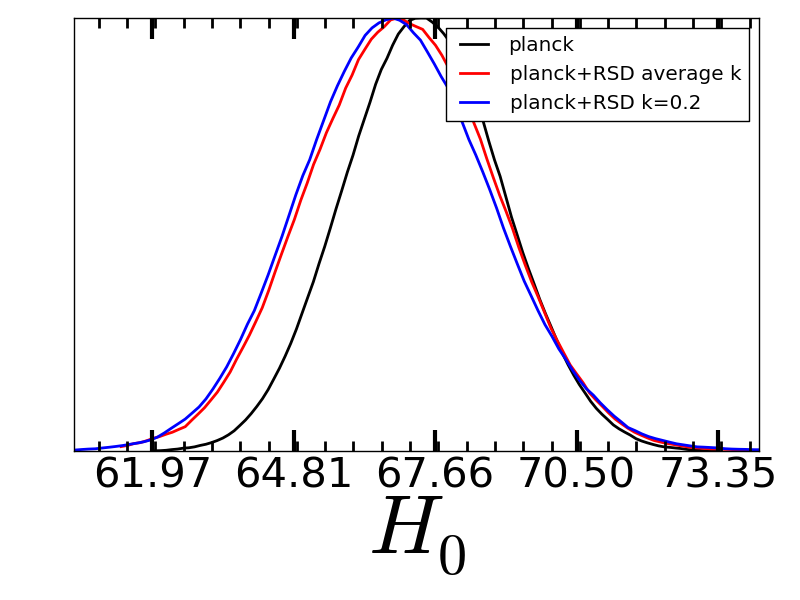
\includegraphics[width=0.3\textwidth]{plots/planck-RSD-Lind-H0.png}
%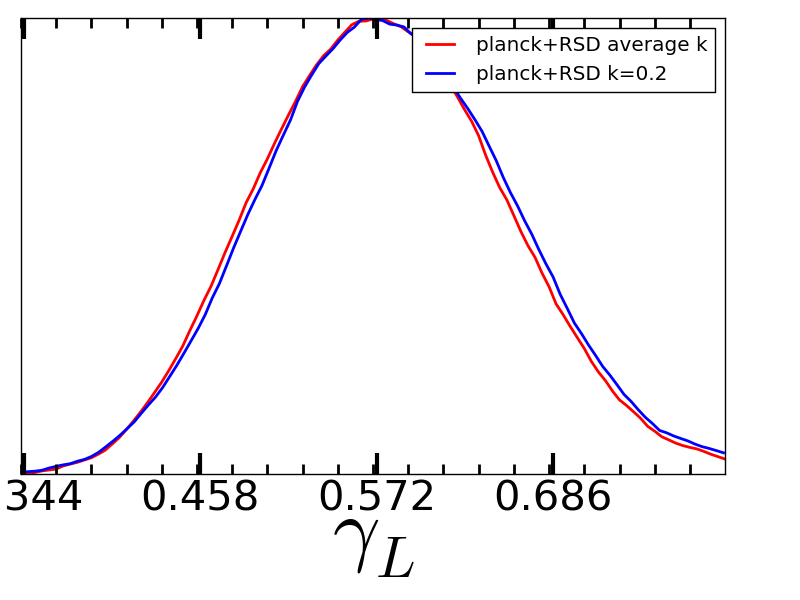
\includegraphics[width=0.3\textwidth]{plots/planck-RSD-Lind-Linder_gamma.png}
%\caption{Linder's $\gamma_L$ parametrization: This has one extra parameter $\gamma$ which is fixed at 0.545 for GR. This shows a higher shift in $\tau$ and hence predict a lower redshift of reionization $z_{re}$. This predicts $\gamma=0.575 \pm 0.077$ which is $0.4\sigma$ from GR prediction.
%}
%\end{figure*}

\subsection{$f(R)$ theory}
\begin{figure}
    \begin{center}        
        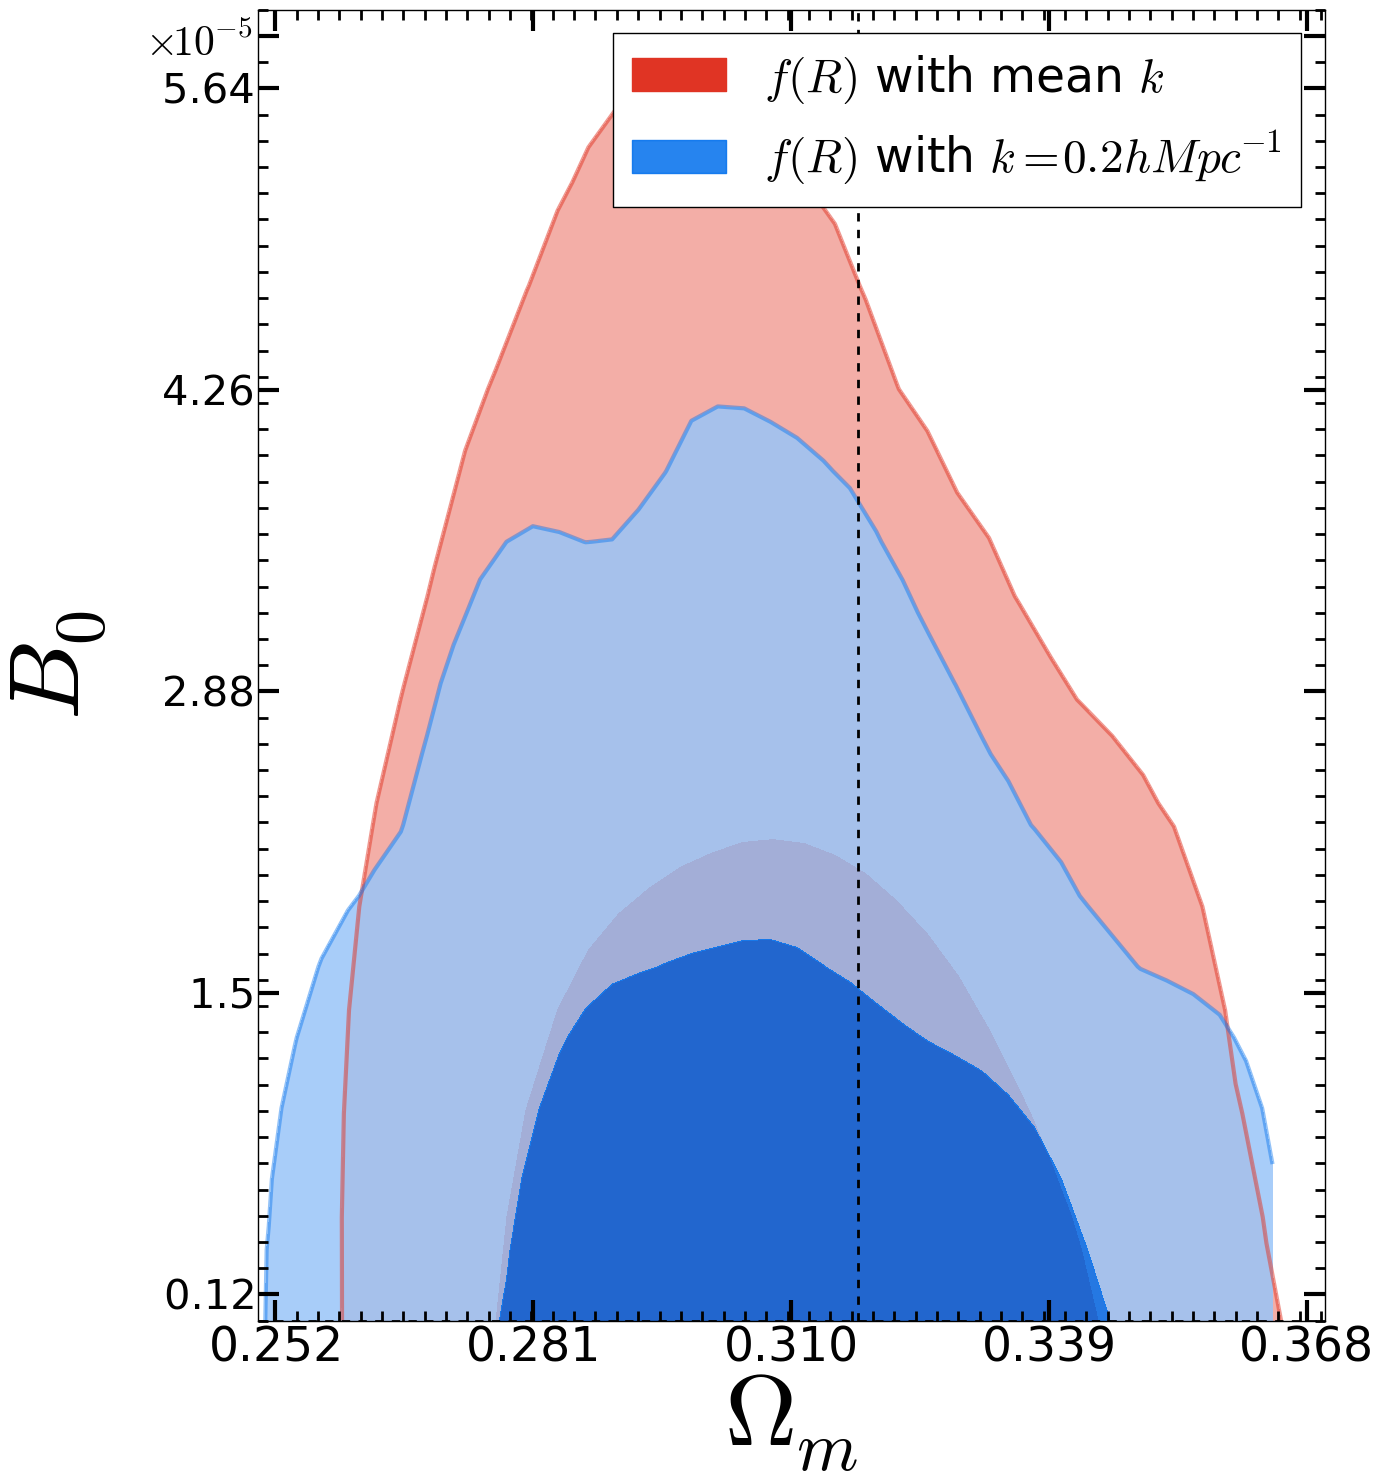
\includegraphics[width=0.5\textwidth]{plots/Like-2D/fR-omegam-lambda1_2_2D.png}
     \end{center}
     \caption{fR}
     \label{fig:fR}
\end{figure}

We consider one parameter ($B_0$) model of $f(R)$ gravity. The parameter $B_0$ parameterize the deviation from $\Lambda$CDM-GR. The model approaches GR when $B_0$ is zeros. We find that the $B_0$ parameter is constrained to be $B_0 < 1.5 \times 10^{-5}$ ($1\sigma$ C.L.). Compare the result with literature.


%\begin{figure*} 
%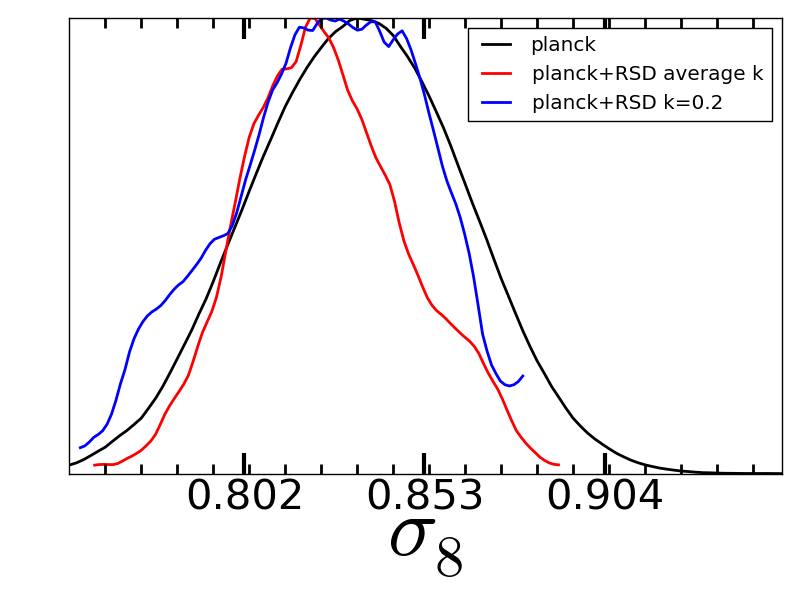
\includegraphics[width=0.3\textwidth]{plots/planck-RSD-fR-sigma8.png}
%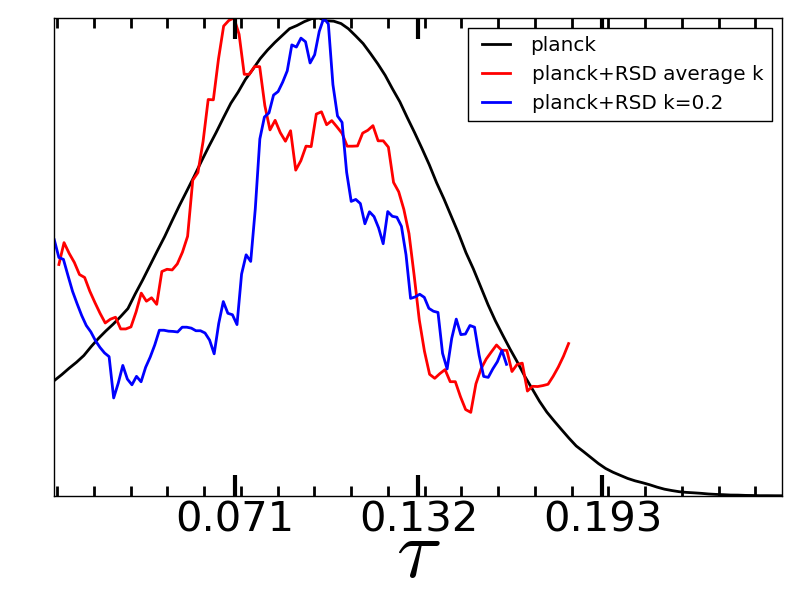
\includegraphics[width=0.3\textwidth]{plots/planck-RSD-fR-tau.png}
%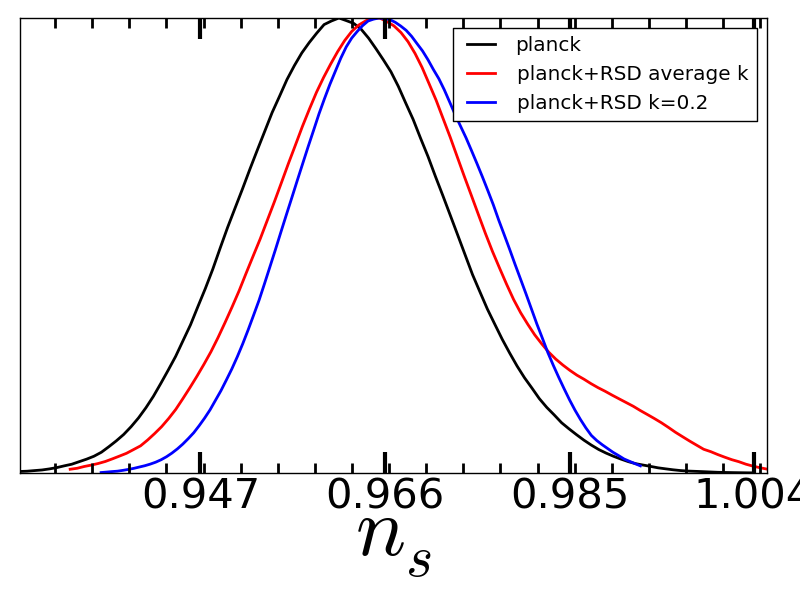
\includegraphics[width=0.3\textwidth]{plots/planck-RSD-fR-ns.png}
%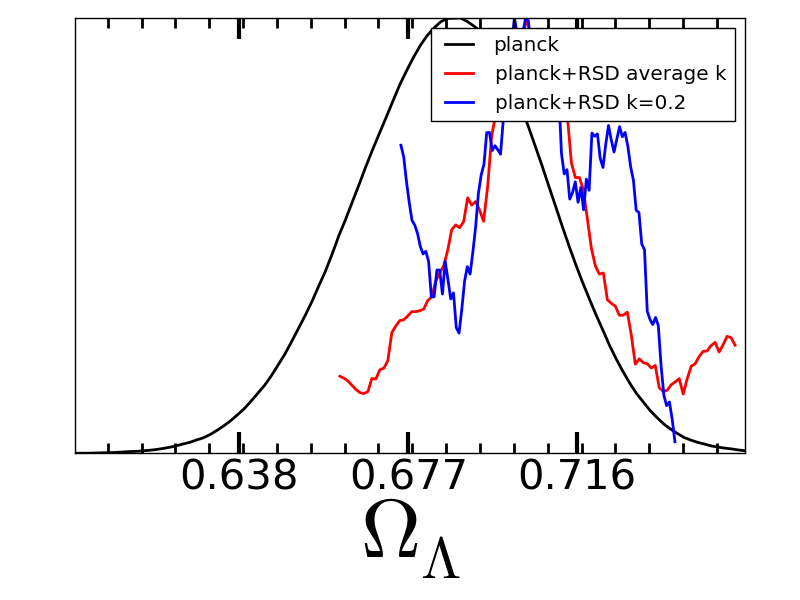
\includegraphics[width=0.3\textwidth]{plots/planck-RSD-fR-omegal.png}
%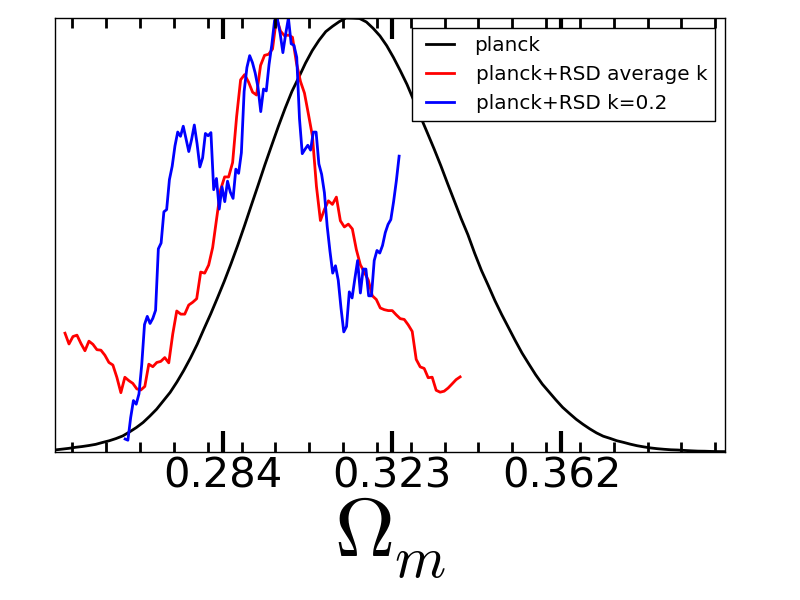
\includegraphics[width=0.3\textwidth]{plots/planck-RSD-fR-omegam.png}
%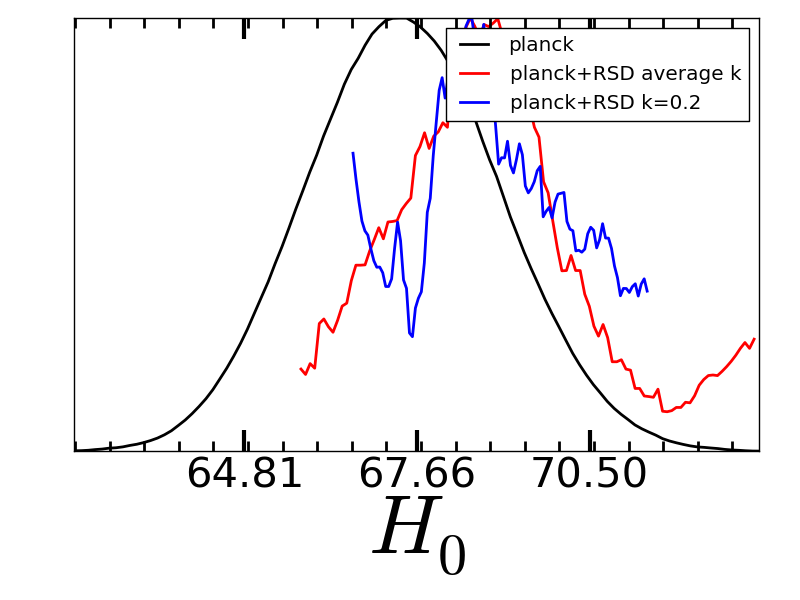
\includegraphics[width=0.3\textwidth]{plots/planck-RSD-fR-H0.png}
%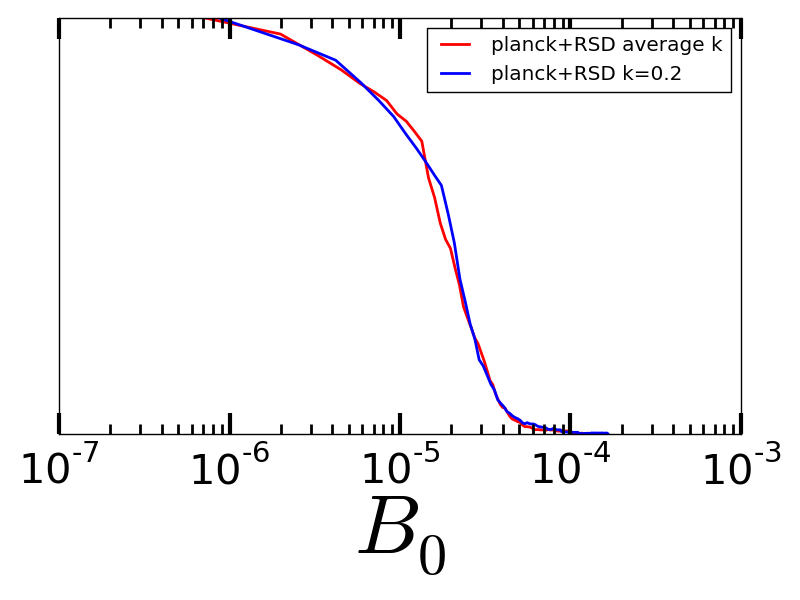
\includegraphics[width=0.3\textwidth]{plots/planck-RSD-fR-lambda1_2.png}
%\caption{$f(R)$ gravity: This case shows very slow convergence and it is still far from convergence.  Although the likelihood for $B_o$ looks smooth. The current value is $B_o =1.2 \times 10^{-5} $ with $\sigma_{B_o}=1.5 \times 10^{-5}$ which gives $1\sigma$ upper limit on $B_o$ as $2.7 \times 10^{-5}$.}
%\end{figure*}